\section{Converting the 1D stellar evolution model to a 3D gas particle distribution}\label{sec:1D_to_3D}

In addition to fundamental parameters such as mass, radius, etc., MESA enables to access the stars internal structure. This information is essential to convert the 1D stellar models into 3D hydrodynamical realizations, providing a more comprehensive understanding of the physical processes involved in \ac{rlof} and the resulting mass transfer in these systems.

When the radius of the outer star exceeds its Roche limit, the 1D stellar evolution model is converted to a collection of \ac{sph} particles. This is accomplished by requesting the radial stellar structure profiles for density, temperature, mean molecular weight, and radius from the stellar evolution code. MESA divides a star into a series of spherical shells, which are represented by arrays in which these parameters are recorded. Following that, I produce a kinematically cold set of $N$ particles of mass $M_{RLOF}/N$ in a uniform spherical distribution. I now scale the particle locations radially to fit the density profile from the star up to its outer radius.

\subsection{Stellar Interior}\label{sub:core}

Because of the usage of equal-mass particles and the high concentration of stellar cores, the majority of the particles, and therefore the maximum resolution, will be in the stellar core, whereas the star's outer edge will be barely resolved. However, I want to investigate the hydrodynamical factors that dominate the star's outer layers in order to gain meaningful insights into the mass transfer process. To achieve that, I replace the stellar high density interior with a single mass point, i.e. core particle, because the interior of the Roche lobe filling star barely affects the dynamics of the outer layers on the short-dynamical timescales associated with \ac{rlof} \citep{deupree2005structure}. This technique not only provides higher resolution of the outer layers but also helps to circumvent computational run time constraints by using less particles. This procedure is coded in the standard AMUSE routine called $star\_to\_sph.py$.
\begin{figure}[H]
    \centering
    \includegraphics[width=0.9\textwidth]{Thesis/graphs/ROLF_density_profile.pdf}
    \caption{Radial density profile of the  $\xi$ Tau outer component at the onset of \ac{rlof} (blue line). MESA's 1D density profile of the tertiary is shown by the solid blue line. The shaded region represents 99.9\% of the star's enclosed mass. The dotted lines depict \ac{sph} models with varied core particle masses, M$_{core}$. The core particles' mass correspond to fractions of 0.1, 0.255, 0.5, and 0.75 of the overall mass of 5.5 M$_{\odot}$, respectively. The core particle of each model is depicted by a larger point at it respective color.}
    \label{fig:stellar_density_ROLF}
\end{figure}
The core particle's mass is unrelated to the mass of the hydrogen-exhausted stellar core, but rather a solution to the computational challenges of modeling big stars without changing the stellar envelope's behavior. Furthermore, it as a pure gravitational point mass with no pressure or internal energy. I investigate core masses corresponding to different percentages of the star's mass at the onset of \ac{rlof}, which are listed in \cref{tab:core_masses_ROLF}. 
\begin{table}[H]
    \centering
    \begin{tabular}{| c |}
       M$_{core}$  \\
       \hline
       10\% M$_{RLOF}$\\
       25\% M$_{RLOF}$\\
       50\% M$_{RLOF}$\\
       75\% M$_{RLOF}$
    \end{tabular}
    \caption{ Different core masses for the 3D hydrodynamical model of the tertiary at the beginning of \ac{rlof}}
    \label{tab:core_masses_ROLF}
\end{table}
Lower core masses, M$_{core}$ $\leq$ 0.2M$_{RLOF}$, retain the problematic high density in the core, but larger core masses, M$_{core}$ $\geq$ 0.4 M$_{RLOF}$, cause the density in the envelope to depart significantly from the stellar structure model. This trend is apparent in \cref{fig:stellar_density_ROLF}. I adopt M$_{core}$ = 0.255 M$_{RLOF}$ (= 1.4 M$_{\odot}$), which successfully overcomes the problematic high density inner stellar region and is in good agreement with envelopes' density profile.

After investigating different number of particles, $N$, I adopt $N=50000$  due to the fact that higher $N$ numbers does not offer a significant improvement in resolving the outer layers of the star, while increase significantly the computational run time of the simulations.  Hence, each particle represents $M_{RLOF}/N = 11 \times 10^{-4}$ M$_{\odot}$ of gas.

\subsection{Stellar envelope: Convective case}\label{sub:envelope_conv}

Following the distribution of particles based on the 1D density profile of the tertiary, I need to accurately specify important thermodynamic properties of the envelope (3D model), such as specific internal energy and specific entropy. Because the pressure of a gas is related to its internal energy, I need to examine the pressure sources in the envelope. In general, the pressure in a non-degenerate stellar interior will be given as 
\begin{equation}\label{eq:pressure}
    P(r) = \frac{1}{3} \alpha T(r)^4+ \frac{\mathcal{R}}{\mu(r)} \rho(r) T(r)
\end{equation}
where $\alpha$ and $\mathcal{R}$ are the radiation and universal gas constants, respectively. The first term in \cref{eq:pressure} is the radiation pressure exerted by photons and it will be dominant for massive hot stars, while it can be neglected for cool stars \citep{pols2011stellar}.

Although, I do not expect the radiative component to be dominant in a $5.5$ M$_{\odot}$ star, I verify this assumption. In \cref{fig:eos}, I present, in black dashed lines, the boundaries between different sources of pressure. The coloured regions mark what pressure source dominate the equation of state in the considered regime of temperature and density, namely the radiation, the ideal gas or the (non-relativistic / relativistic) electron degeneracy pressure. The blue line corresponds to the internal structure of the tertiary at moment of \ac{rlof}. Starting from right to left, I follow the density and temperature of the star from the core to its surface. The black $x$ indicate, for decreasing $\rho$, the part of the star containing 1.375 M$_{\odot}$, 2.75 M$_{\odot}$, 4.125M$_{\odot}$ and 5.5 M$_{\odot}$, respectively. These values correspond to 25\%, 50\%, 75\% and 100\% of the star's enclosed mass.
\begin{figure}[H]
    \centering
    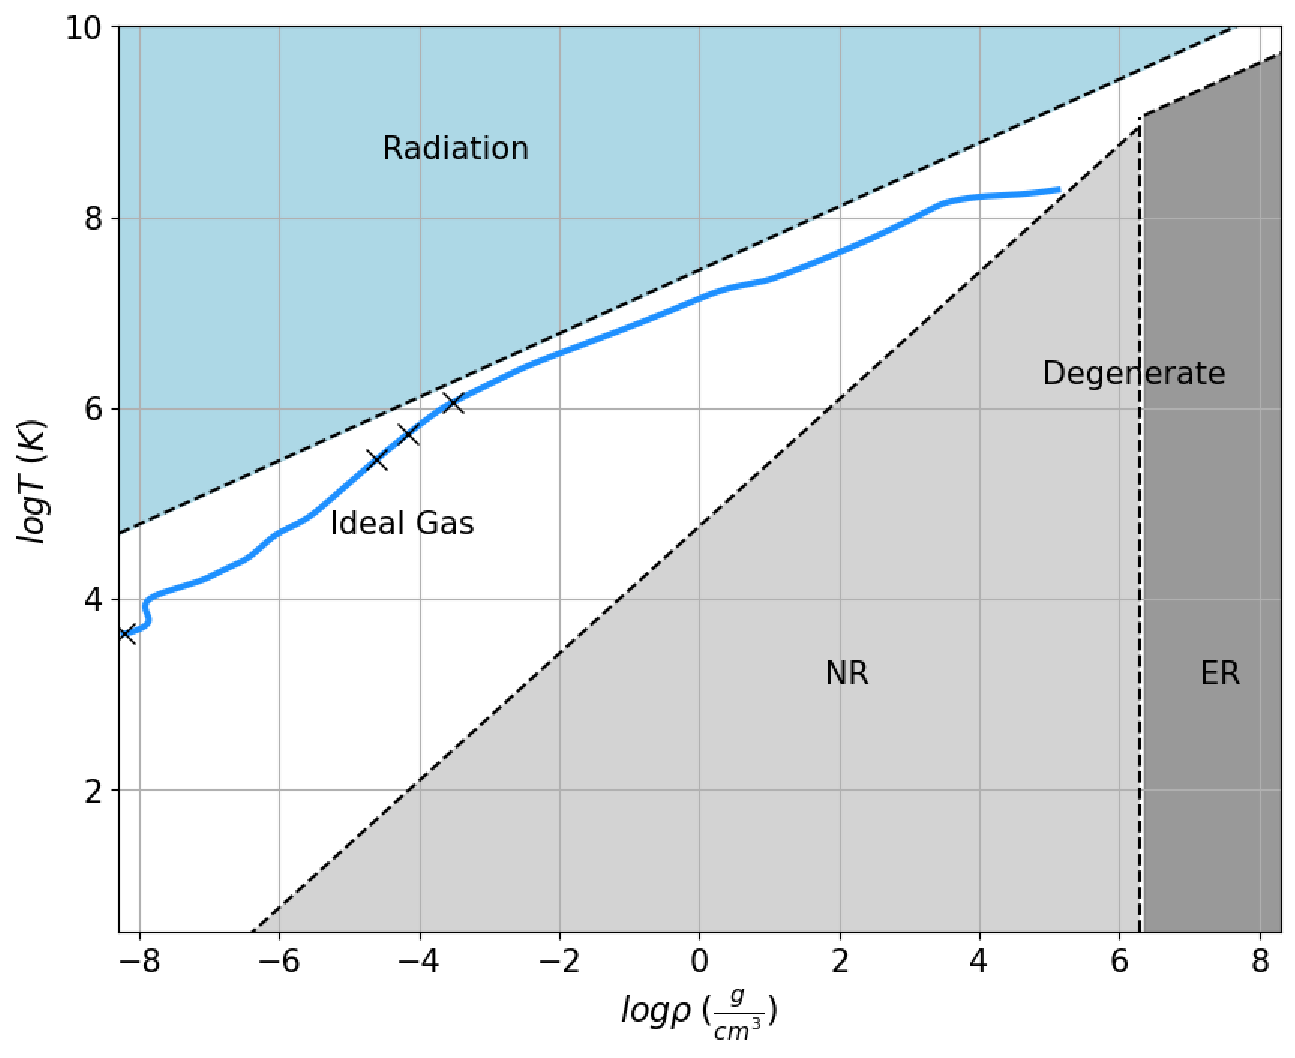
\includegraphics[width=0.9\textwidth]{Thesis/graphs/eos.pdf}
    \caption{ The radial structure of the outer star at the moment of \ac{rlof} in the  temperature-density plane. I calculate the stellar profile using MESA \citep{paxton2010modules,paxton2013modules,paxton2015modules,paxton2019modules}.}
    \label{fig:eos}
\end{figure}
At the moment of \ac{rlof} the pressure within the envelope is dominated by the ideal gas component, see \cref{fig:eos}. Thus I can indeed neglect the radiative part of \cref{eq:pressure}. Using
\begin{equation}\label{eq:pressure_ideal_gass}
    P(r) =  \frac{\mathcal{R}}{\mu(r)} \rho(r) T(r)
\end{equation}
each particle is allocated a unique specific internal energy based on the temperature and mean molecular mass profiles:
\begin{equation}\label{eq:internal_energy}
    u(r) = \frac{3}{2} \frac{k_B T(r)}{\mu(r)},
\end{equation}
where $k_B$ is the Stefan-Boltzmann constant, $T(r)$ and $\mu(r)$ the temperature and mean molecular mass profiles, respectively.

The particles at this point are kinematically cold meaning that their specific kinetic energies are zero and only their internal and potential energies contribute to the total energy of the gas. This is illustrated in \cref{fig:kinetic_internal_energies}, where I present 2D maps of the kinetic and internal particle energies, respectively.
\begin{figure}[H]
    \centering
    \begin{subfigure}{.5\textwidth}
    \centering
    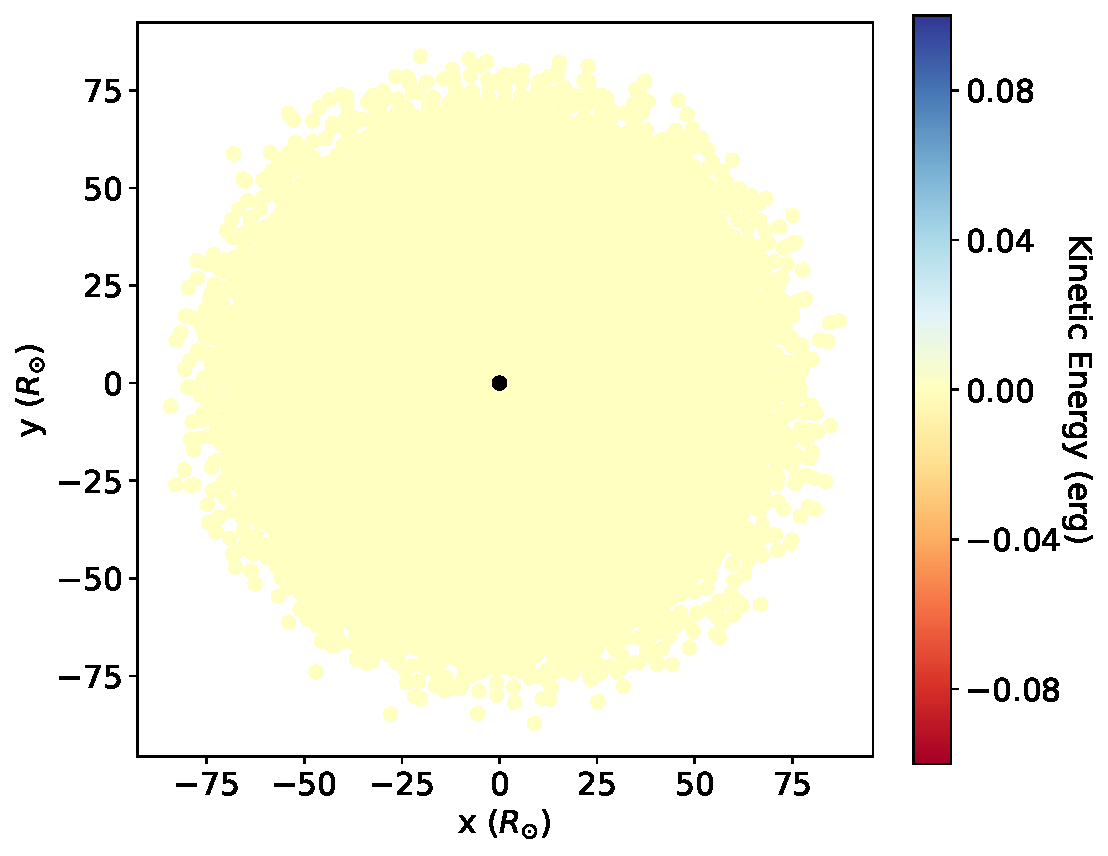
\includegraphics[width=0.9\textwidth]{Thesis/graphs/tertiary_kin_energy_before_relaxation.pdf}
    \label{fig:mass_loss}
    \end{subfigure}%
    \begin{subfigure}{.5\textwidth}
    \centering
    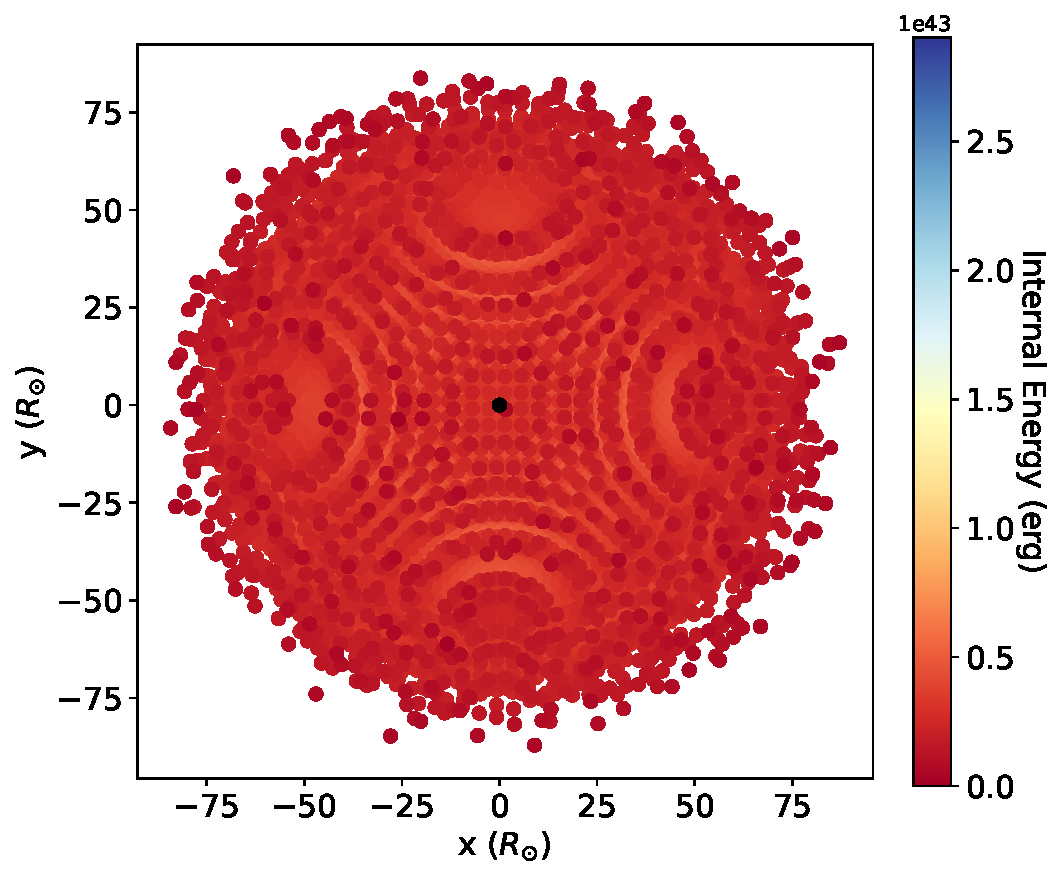
\includegraphics[width=0.9\textwidth]{Thesis/graphs/tertiary_internal_energy_before_relaxation.pdf}
    \label{fig:radius_profile}
    \end{subfigure}
    \caption{ Kinetic and internal energies of the gas particles after converting the 1D stellar evolution model to a 3D gas particle distribution. The black point corresponds to the core particle which is a pure gravitational point mass with no pressure or internal energy.}
    \label{fig:kinetic_internal_energies}
\end{figure}
Another important parameter of the gas is its specific entropy. It is often mathematically simpler, although not formally necessary, to define an entropic variable $A$. The entropic variable $A$ is closely linked (but not identical) to the specific entropy and it is defined as
\begin{equation}\label{eq:entropic_variable}
    A(r) \equiv \frac{P(r)}{\rho(r)^{\gamma_{ad}}}
\end{equation}
where $\gamma_{ad}$ is the adiabatic index, and $P(r)$ and $\rho(r)$ the pressure and density profiles, respectively. 

The evaluation of the original entropic profile $A(r)$ of the stellar envelope is not trivial and one needs to consider the relevant pressure sources, see \cref{eq:pressure}. In a radiation-dominated gas, $\gamma_{ad} = 4/3$ is a more suitable adiabatic index (this is in general true when extremely relativistic particles dominate), while for a mixture of gas and radiation, $4/3 \leq \gamma \leq 5/3$. However, at the moment of \ac{rlof}, see \cref{fig:eos}, ideal gas is the dominant radiation pressure source, thus considering \cref{eq:internal_energy} and \cref{eq:entropic_variable}, I calculate the entropic profile $A(r)$ with $\gamma = 5/3$, such as:
\begin{equation}\label{eq:entropic_variable_2}
    A(r) = \frac{2}{3} u(r) \rho(r)^{-2/3}.
\end{equation}

\subsection{Stellar envelope: Radiative case}\label{sub:envelope_rad}

In the previous subsections I showed how I model $\xi$ Tau's outer component. The presented method works pretty well due to the fact that the envelope is convective at the onset of \ac{rlof}. I tested the scenario of \ac{rlof} occurring at different phases of the evolution, when the envelope is radiative, and for different initial stellar masses. Hence, I present the additional parameters that need to be considered in the case of a radiative envelope. These key points can be incredibly valuable and time-saving for future work using the same method.

Low-mass, thus cold, stars have convective envelopes during their evolution, while massive stars with M$>16$M$_{\odot}$ remain with a radiative envelope pretty much until the end of their lives. Intermediate- and high-mass stars' envelopes (M  $<16$M$_{\odot}$) can be either convective or radiative depending on the evolutionary phase in which \ac{rlof} occurs, see \cref{sec:single_star_evolution}. 
\begin{figure}[H]
    \centering
    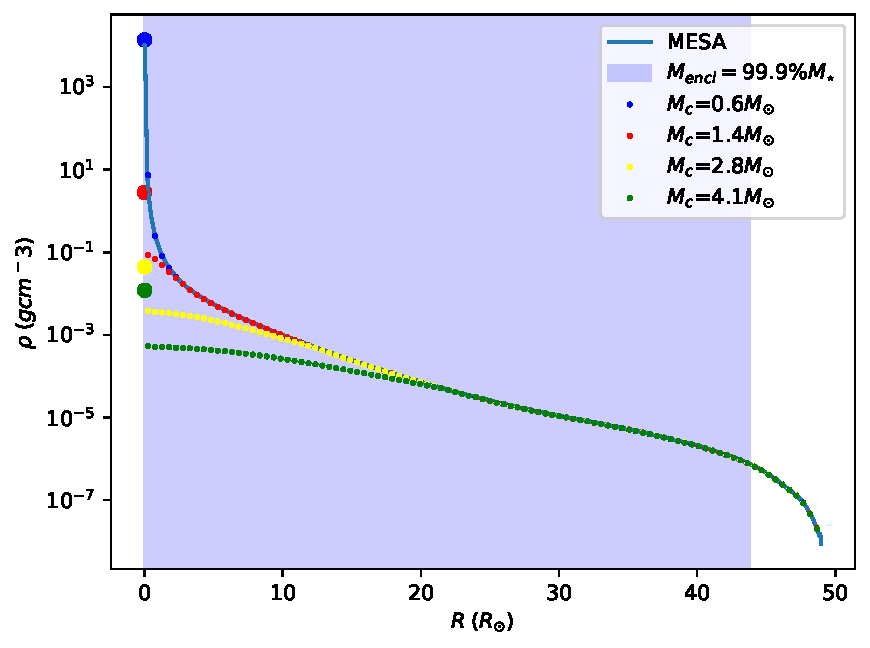
\includegraphics[width=0.9\textwidth]{Thesis/graphs/density_profile_radiative_envelope.pdf}
    \caption{Radial density profile of the  $\xi$ Tau outer component at $t=78.3$ Myr (blue line), when the star is in its helium-burning phase and has a fully radiative envelope. MESA's 1D density profile of the tertiary is shown by the solid blue line. The shaded region represents 99.9\% of the star's enclosed mass. The dotted lines depict \ac{sph} models with varied core particle masses, M$_{core}$. The core particles' mass correspond to fractions of 0.1, 0.255, 0.5, and 0.75 of the overall mass of 5.5 M$_{\odot}$, respectively. The core particle of each model is depicted by a larger point at it respective color.}
    \label{fig:density_profile_radiative}
\end{figure}
The density within a convective envelope falls of with pressure $\rho \propto P^{1/\gamma_{ad}}$, see \cref{eq:adiabatic_eos}. If the envelope is stable against convection, the density gradient must vary more steeply with pressure than for an adiabatic change by definition. This means that radiative envelopes are less dense in the outer layers and more centrally concentrated than convective envelopes \cite{pols2011stellar}. This is reflected in \cref{fig:density_profile_radiative}, where I plot the tertiary's radial density profile at $t=78.3$ Myr, when the star is in its helium-burning phase and has a fully radiative envelope, see \cref{fig:kippen_plot}.

Modeling the radiative envelope case is more challenging. From the computational point of view, the problem branches in to two sub-problems. First, a comparison between \cref{fig:stellar_density_ROLF} and \cref{{fig:density_profile_radiative}} immediately reveals the difference in scales. More specifically, in the radiative case someone needs to resolve 6-8 orders of magnitude in density. In \cref{fig:density_profile_radiative}, I use $N=10^6$ particles and still the outer layers of the star are not very well resolved. This is a direct consequence of the density's profile high steepness and the use of equal mass particles. In general, the use of equal mass particles provides good resolution in high-density regions, however, only poorly resolves low-density regions. Second, using $N$ of 6 orders of magnitude, will result in extremely long computational time, as the CPU simulation time is not linear function of $N$, but rather the CPU time increases with the number of \ac{sph} particles as $NlogN$.

The problematic steepness of the density profile becomes more severe for high-mass stars. Additionally, as stellar mass grows so does the importance of radiation pressure. From a physics standpoint, someone must estimate the importance of radiation in order to accurately define the thermodynamic properties of the gas using \cref{eq:pressure}, \cref{eq:entropic_variable} and a proper adiabatic index, $\gamma_{ad}$.

In conclusion, the method is preferable for modeling low- and intermediate-mass stars with convective envelopes. For high-mass stars, even if the thermodynamic properties of the gas are defined properly, the intrinsic steepness of the density profile will remain.  Hence, a very high number of \ac{sph} particles are needed to resolve the stellar envelope, which result in very long computational times. 

